%%
%% 研究報告用スイッチ
%% [techrep]
%%
%% 欧文表記無しのスイッチ(etitle,eabstractは任意)
%% [noauthor]
%%

%\documentclass[submit,techrep]{ipsj}
\documentclass[submit,techrep,noauthor]{ipsj}



%\usepackage[dvips]{graphicx}
\usepackage{latexsym}
\usepackage[dvipdfmx]{graphicx}
\def\Underline{\setbox0\hbox\bgroup\let\\\endUnderline}
\def\endUnderline{\vphantom{y}\egroup\smash{\underline{\box0}}\\}
\def\|{\verb|}
%

%\setcounter{巻数}{59}%vol59=2018
%\setcounter{号数}{10}
%\setcounter{page}{1}


\begin{document}


\title{ADLogger\\
タスク別時間記録システムの構築の提案}

\etitle{ADLogger:Behavior Modification for ADL Time Management }

\affiliate{Keio}{慶應義塾大学\\
Keio University, Fujisawa, Kanagawa 252--0882, Japan}

\author{助川 友理}{Yuri Sukegawa}{Keio}[suke@ht.sfc.keio.ac.jp]
\author{羽柴 彩月}{Satsuki Hashiba}{Keio}[shiba@ht.sfc.keio.ac.jp]
\author{大越 匡}{Tadashi Okoshi}{Keio}[slash@ht.sfc.keio.ac.jp]
\author{中澤 仁}{Jin Nakazawa}{Keio}[jin@ht.sfc.keio.ac.jp]

\begin{abstract}
私たちは時間を指標に生活を続けており,時間管理を心がける場面は公私双方様々な場面で存在する.特に 朝の支度準備など個人管理の面で時間管理を意識する事は重要である.一方で,「逆算の甘さ」が原因で時間管理に苦手意識のある人は多い.本研究では正確な行動時間把握を目的とするシステム「ADLogger」を提案し,時間管理において重要となる「感覚に依存した見積もりの誤差」「バッファの不備」を回避する事で時間管理行動に対する苦手意識や行動の変化を与える事を目指す.具体的には実測値の平均時間及び余白時間を元に合計時間予測を提案する.「ADLogger」では実測値の記録及び標準偏差の信頼範囲に基づくバッファを考慮した必要時間自動計算機能を搭載している.「ADLogger」導入前後で見積もり時間や苦手意識の変化が現れるかを調査すべく大学生 20 名を被験者として約4週間に渡る評価実験を行った.結果全ての被験者においてタスク・総合時間の時間もしくは\%比において実態の時間が見積もりの時間予測に合いやすくなり,全体の実測値の分布のばらつきを縮小する効果が示唆された.
\end{abstract}


\begin{jkeyword}
時間知覚 (認知),遅刻,行動変容,メタ認知,セルフマネジメント,Well-being Computing
\end{jkeyword}

\begin{eabstract}
There are many situations in which we need to care about time management, both in public and private life such as getting ready in the morning. However, there are many people who are not good at time management because of lacking extra time as buffer. In this study, we propose an iOS application “ADLogger” that aims to estimate the time needed to complete a task. “ADLogger” is a system that expects how much time you may spend to the task and define the accurate buffer according to your time log data to avoid ”errors in estimation depending on the senses” and ”inadequate buffers,” which are important in time management. Plus, the system is designed to manage time by including sufficient margin time in objective measurements and preparation time. We conducted a four-week evaluation experiment with 20 university students to investigate whether the estimation time and the sense of difficulty change before and after the introduction of this system. The results suggested that the system reduced the variance between the estimation time and the actual time. On the other hand, some of the subjects reduced the estimation time in the direction of reducing the margin, and the large individual differences remained as problems. In the future, it will be necessary to change the functions and optimize the estimation time according to the type of user.
\end{eabstract}

\begin{ekeyword}
Time Perception, Tardiness, Behavior Modification, Metacognition, Self-Management, Well-being Computing
\end{ekeyword}

\maketitle

%1
\section{はじめに}
時間は出来事や変化を認識するための基礎的な概念である\cite{history}.
%\cite{Taylor1911}.
プロジェクト管理においては「感覚に依存した見積もりの誤差」「バッファの不備」による計画の失敗を非常に懸念する.
%\cite{innopm}.
こうした失敗を避けるべく現在のプロジェクト管理は主に1940年代から考案された多くの手法やフレームワークを参考にし実際のビジネスに応用する動きが多くみられる.
%\cite{EORMS}.

%ADHDとの関連性も簡潔に書く?
また,近年では生産性だけではなく時間管理能力と個人のパフォーマンスやストレスと言った関連性を考える研究も存在する.
例えば表\ref{tb:dif}の様にそれぞれ定義した質問紙を用いた研究では
%\cite{Imura2016}
時間管理能力の高い人はパフォーマンスの高さ\cite{Britton1991}\cite{Trueman1996}やストレスの低さ\cite{Macan1994}も伴うという仮説が立てられている\cite{Claessens2007}.

\begin{table*}[tb]
\setbox0\vbox{\large

\begin{center}
\caption{時間管理の定義}
\ecaption{Definition of time management}
\begin{tabular}{|c|c|c|} \hline
Macan(1994) & Britton\&Tesser(1991) & Bond\&Feather(1988)  \\ \hline \hline

\begin{tabular}{c}
時間を管理するための技術
\end{tabular}
 & 
\begin{tabular}{c}
 知的な生産性を最大化すること\\を意図した実践
\end{tabular}
&
\begin{tabular}{c}
 個人が自身の時間を\\どの程度構成し\\目的にかなった様に\\できているかと知覚している程度
\end{tabular}
\\ \hline
Time Management Behavior Scale & Time Management Questionnaire & Time Structure Questionnaire  \\ \hline
\end{tabular}
\end{center}
}

\centerline{{\hbox to.9\textwidth{\hss\box0\hss}}}
\label{tb:dif}
\end{table*}


時間管理は朝の支度準備など個人管理の側面において時間を管理する機会は日常生活の中でも数多く存在する.
しかし個人による時間管理は完璧であるとは言い難い.
例えば文京学院大学による遅刻の状況の調査によると授業・友達の待ち合わせ共に「逆算の甘さ」によって遅刻すると考えている人が多数を占める\cite{bunkyo}.

\section{目的}
逆算を補助する事で個人の時間管理の精度を向上させ,
時間管理能力やパフォーマンスの向上及び苦手意識やストレス軽減といった精神面に効果が期待できる.
本研究は朝の支度準備における時間管理の失敗に関する仮説を提案・分析した上で,行動時間の実測値記録及び必要時間の簡算出補助を提案し時間管理の精度向上対し変化を与える事を目的としている.

%2

\section{関連研究}
\subsection{時間管理の定義}
時間管理の定義は多岐にわたる.
著名なものとしてLakeinの定義\cite{Lakein1989}が挙げられる(表~\ref{tb:Lakein}).
Lakeinは個人管理という位置付けで時間管理に言及し,下記の4項目に則り時間管理を遂行していく重要性を説いた.

\begin{table}[htb]
\begin{center}
  \caption{Lakeinによる時間管理の定義}
  \begin{tabular}{|l|l|} \hline
   1 & すべきことを決定する \\ \hline
   2 & 達成するための目標を設定する \\ \hline
   3 & 優先順位を決める \\ \hline
   4 & 取り組む課題のプランニングを作る \\ \hline
  \end{tabular}
  \label{tb:Lakein}
\end{center}
\end{table}

Claessens らは,先行研究の定義を俯瞰した上で,時間管理を「目標を達成するために時間を効果的に使用する行動」と定義し時間管理の行動を更に以下の3つに分類した\cite{Claessens2007}(表 ~\ref{tb:Claessens}).


\begin{table}[htb]
\begin{center}
  \caption{Claessens et al. による時間管理の定義}
  \begin{tabular}{|l|l|} \hline
   時間アセスメント行動(time assessment behavior): \\ ~~~過去,現在,未来の時間を認識し,\\時間の使い方に関して認識する事 \\ \hline
   プランニング行動(planning behavior): \\  ~~~時間を効率的に使用する事を目的とする事 \\ \hline
   モニタリング行動(monitoring behavior): \\ ~~~行動中における時間の配分のモニタリング\\・不測の事態へのリスクヘッジ等 \\ \hline
  \end{tabular}
  \label{tb:Claessens}
\end{center}
\end{table}

\subsection{時間管理の先行研究}
時間管理研究は大きく分けて時間管理がもたらす効果の研究と時間管理能力に関する研究の2種類に分けられる.
時間管理能力の研究では主に見積もり時間の精度に関して議論されている.
与えられた課題の時間や経験の有無\cite{Roy2007}などと言った見積もりの精度は大きく分けて課題に対するものと時間評価における知覚時間の歪み\cite{Oguro1961}\cite{Murakami2016}など被験者の個人差によるものの2種類存在しているが,原因として記憶との関連性が考えられている.

正確な見積もりを計算する手法は主に大規模プロジェクト向けに提案される事が多い.
例えばPERT(Program Evaluation and Review Technique)では個々のタスクの見積もりを予測する手法である「三点見積もり法」が考案されている.
三点見積もり法はタスク完了に要する時間の最良見積もり(期待時間)値を$T_{E}$,タスク完了に必要な最小時間の予測(楽観的時間)を$O$,タスク完了に必要と思われる最頻値の見積時間(最確時間)を$M$,タスク完了に必要な最大時間の予測(悲観的時間)を$P$とすると,数式(\ref{pert})の様に見積もりを行う.ただし,三点見積もり法は参加者が複数人いる長期の大型プロジェクトに対する適切な管理方法であり,参加者の多くないプロジェクトでは最可能値だけを使用した見積りのほうが正確である場合がある\cite{Kato1965}.
\begin{equation}
\label{pert}
T_{E} = (O + 4M + P) /6
\end{equation}

\subsection{時間管理の評価方法}
時間管理の評価手法は複数存在する.例えば被験者に時間の長さを教示し,その長さを産生させる時間産生法(時間作成法)(time production),
被験者が時間を経験した後に体験時間を再生させる時間再生法(time reproduction),
経過した時間間隔を言語的に評価する言語的時間評価法(verbal time estimation)などがある\cite{Oguro1961}.

\subsection{時間管理補助システムの分類}
日常生活動作(Activities of Daily Living;ADL)とは,人が日常生活において繰り返す,身の回りの活動や動作のことである.具体的には,身の回りの動作(食事,更衣,整容,排泄,入浴の各動作),移動動作,その他生活関連動作(家事動作,交通機関の利用等)を指す\cite{Sakai2003}.
朝の準備支度は日常生活動作が複数集まったものであると言える.
今日では日常生活動作を基調とし,身近な時間管理をサポートするシステムが複数開発されている.
まず,身近な時間管理をサポートするシステムにはトップダウン式のものとボトムアップ式のものがある.
トップダウン式は予め秒数が固定されたルーティンに沿って時間を遂行する事を補助するものであり,
例えばルーチンタイマー(図~\ref{fig:routine})などが挙げられる.

\begin{figure}[hb]
	\begin{center}
	\fbox{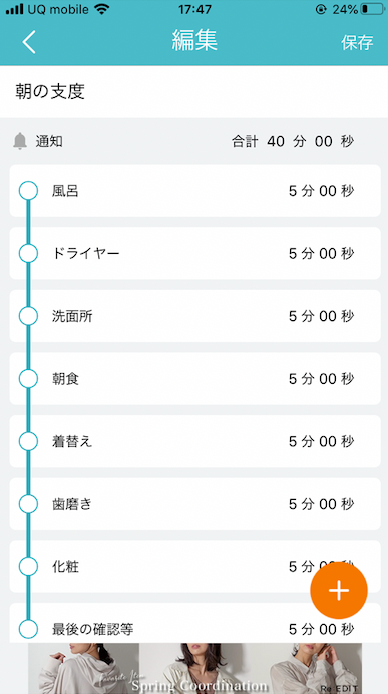
\includegraphics[width=5cm]{images/2/routine.png}}
		\caption{ルーチンタイマーの行動設定例}
		\label{fig:routine}
	\end{center}
\end{figure}

\begin{figure*}[tb]
\setbox0\vbox{\large
\hbox{\
	\fbox{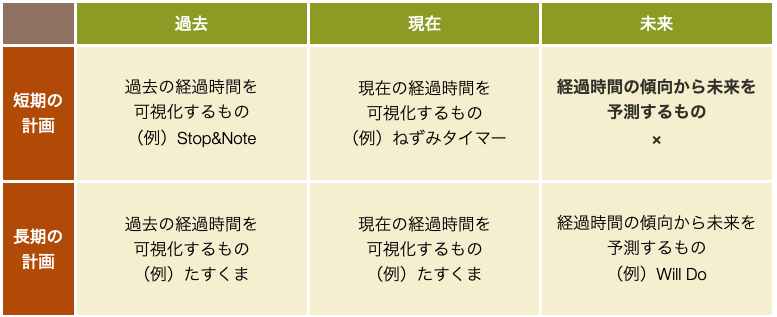
\includegraphics[width=12cm]{images/2/bottom.png}}	
}}
\centerline{{\hbox to.9\textwidth{\hss\box0\hss}}}
\caption{ボトムアップ式の時間管理システムに関する分類}
\ecaption{Double column figure.}
\label{fig:bottomup}
\end{figure*}

一方,ボトムアップ式はタスク毎の経過時間,若しくは時間の使い方の傾向を可視化する事を主眼としているものである.
ボトムアップ式の時間管理システムは図~\ref{fig:bottomup}の様に大別が可能である.
尚,図中の定義された「長期・短期」の区分は時間管理質問紙\cite{Britton1991}に則った.

過去型は行動をタスク別に計測を行う事で過去自分の使った時間を記録し,可視化する事で振り返りに役立てるシステムである.
例えば日毎の時間傾向を可視化するたすくま(図~\ref{fig:taskuma}))といったシステムが挙げられる.

現在型はある時間からの経過時間を可視化する事によって現在の経過時間把握を補助するシステムである.
所謂ストップウォッチは勿論の事,例えば時間の流れをイラストで表現するもの(ねずみタイマー(図~\ref{fig:mouse}))などが挙げられる.
\begin{figure}[ht]
\begin{center}
\begin{tabular}{c}
  	\begin{minipage}[b]{0.5\linewidth}
	\begin{center}
		\fbox{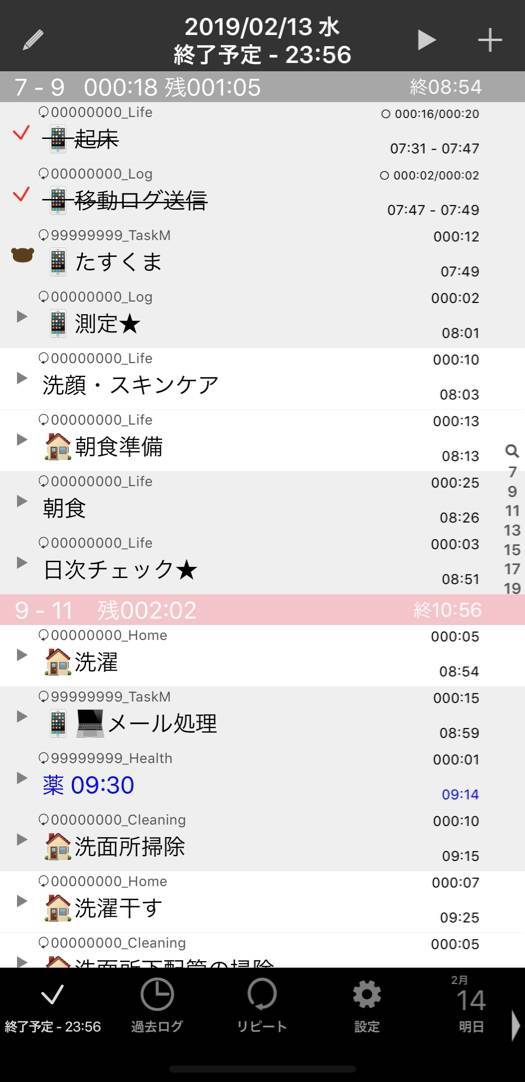
\includegraphics[width=5cm]{images/2/taskuma.png}}
		\caption{たすくまによる一日の可視化}
		\label{fig:taskuma}
	\end{center}
  	\end{minipage}
\\
  	\begin{minipage}[b]{0.5\linewidth}
	\begin{center}
		\fbox{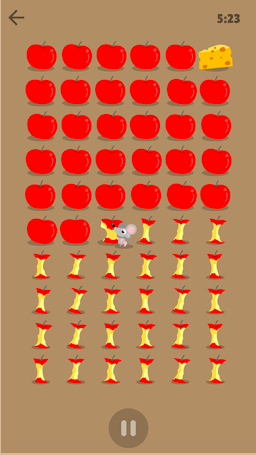
\includegraphics[width=5cm]{images/2/mouse.png}}
		\caption{ねずみタイマーによる経過時間の可視化}
		\label{fig:mouse}
	\end{center}
  	\end{minipage}
\end{tabular}
\end{center}
\end{figure}

\begin{figure}[ht]
\begin{center}
\begin{tabular}{c}

	\begin{minipage}[b]{0.5\linewidth}
	\begin{center}
		\fbox{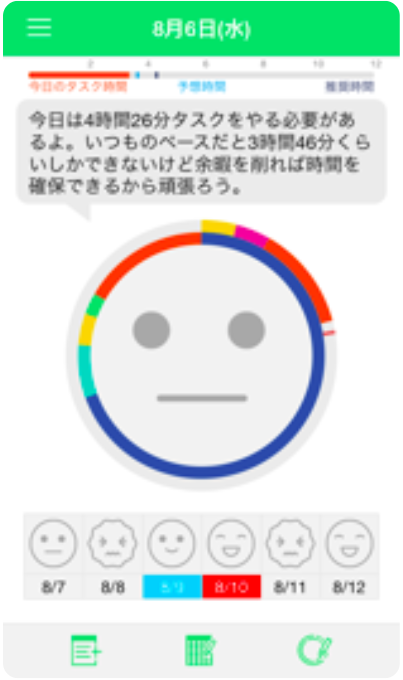
\includegraphics[width=5cm]{images/2/willdo.png}}
		\caption{WillDoによる未来予測}
		\label{fig:will}
	\end{center}
  	\end{minipage}
	
\end{tabular}
\end{center}
\end{figure}

未来型は行動をタスク別に計測する事によって自分の時間傾向をシステム側が把握し,未来自分がどうなるかを予測するシステムである.
この方向性を持つシステムは他の型に比べ現在限られているものの,例えばWillDo(図~\ref{fig:will})が挙げられる.
WillDoは一日の行動を記録することによって,特定のプロジェクトが目標達成までに毎日どれだけかけるべきかを提示する.

\subsection{先行研究からの問題意識}
学術面として最適な見積もりを考える手法は大規模なプロジェクト向けのものが多く,日常生活動作向けに個人管理として使えるものか十分な検証はなされていない.
特に時間評価は日常生活動作を評価する30分から60分規模の研究が乏しい上,見積もりの誤差が小さくなればどういう効果が現れるかに対して検証する研究はなされていない.
またアプリケーションにおいても図~\ref{fig:bottomup}が示す様に短期間における自分の時間傾向を予測する(未来型)のものは無い.

\section{予備実験}
\subsection{予備実験の概要}
本研究に先立ち,時間の逆算の甘さという現象を実測で分析する予備実験を慶應義塾大学大学生20代男女9人を対象に7日間行った.
まず,被験者にインタビューを行い,時間管理に対し苦手意識があるグループと無いグループの2つにグループ分けを行った.今回9人中6人の被験者は朝の時間管理に対し苦手意識があると答えた.次に,遂行タスクをtodoリスト形式で事前登録を行ってもらった上で図~\ref{tb:Q}の項目を被験日時までに被験者に予想して貰った.また,総所要予測時間1 を $T_{1}$,総所要予測時間2 を$T_{2}$,理想の外出時刻を$I$,外出時刻のタイムリミットを$L$,支度開始時刻を$B$と置いた時の数式\ref{1}及び数式\ref{2}を用いて被験者に対する質問項目から必要時間の予測を行った.最後に,タスク別記録アプリケーションを用いて朝の外出準備行動に関するタスク毎の必要時間予測と実測の比較を行った.タスク別記録アプリケーションは予備実験の為に作成されたiOSアプリケーションである.TODOリスト形式でのタスク名登録,タスクの総時間計測,カラム毎のストップウォッチを用いた各タスクの経過時間の記録が可能である.(表~\ref{fig:yobiapp}参照)

\begin{equation}
\label{1}
 T_{1} = I - B 
\end{equation}

\begin{equation}
\label{2}
 T_{2} = L - B
\end{equation}

\begin{figure}[ht]
\begin{center}
\begin{tabular}{c}

	\begin{minipage}[b]{0.5\linewidth}
	\begin{center}
		\fbox{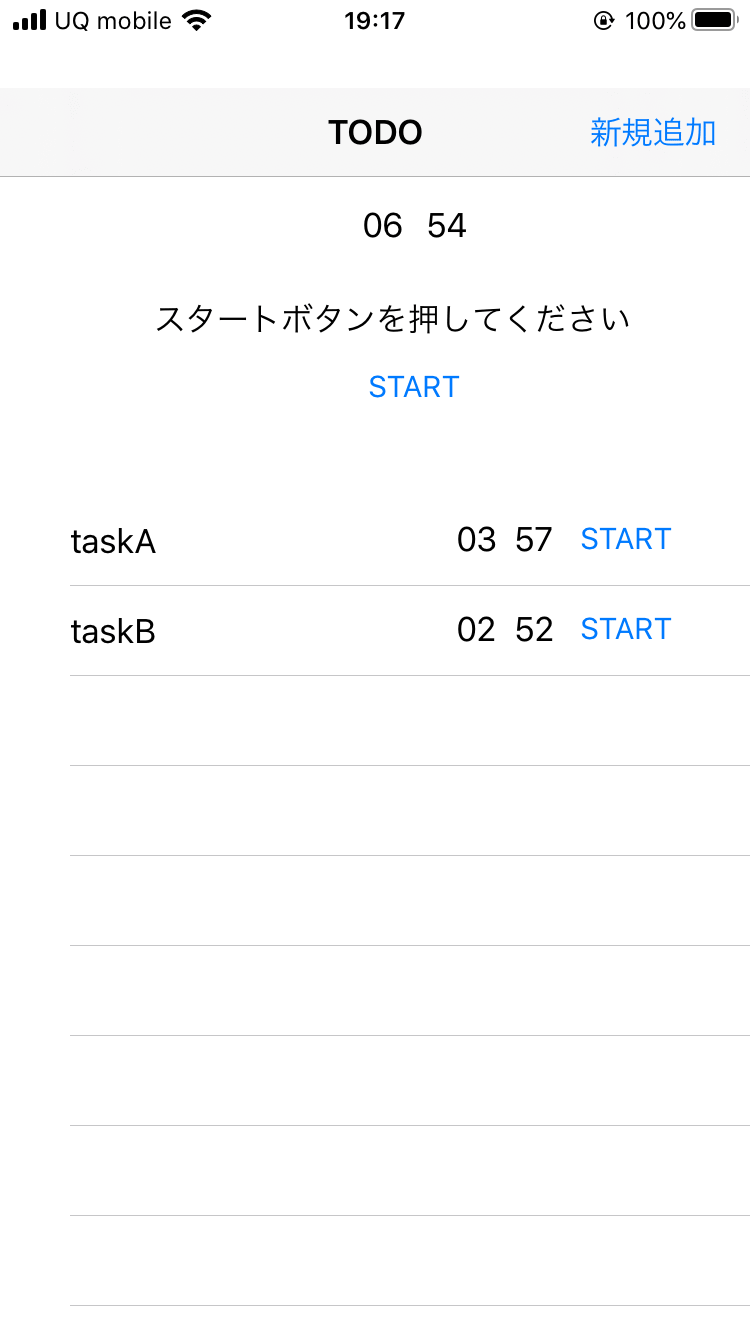
\includegraphics[width=5cm]{images/3/yobi.png}}
		\caption{使用アプリケーション}
		\label{fig:yobiapp}
	\end{center}
  	\end{minipage}
	
\end{tabular}
\end{center}
\end{figure}

\begin{table}[htb]
\begin{center}
  \caption{被験者に対する質問項目}
  \begin{tabular}{|l|l|} \hline
   1 & 支度開始時刻 \\ \hline
   2 & 外出時刻 (理想時刻,外出時刻のタイムリミット) \\ \hline
   3 & 必要タスク \\ \hline
   4 & タスク別所要時間 \\ \hline
  \end{tabular}
  \label{tb:Q}
\end{center}
\end{table}

\subsection{実験結果}
計測日数が0日だった6名(内時間管理に苦手意識のある被験者は5名)を分析対象から除外し,
有効回答者3名(内時間管理に苦手意識のある被験者は1名)を分析の対象とした.
以後被験者A,B,C,と供述する.被験者データとしては被験者Aのみ苦手意識があり.被験者Bのみ3日間,それ以外が1日間のデータが得られた.
図~\ref{fig:re1},\ref{fig:re2}は横軸を被験者名,縦軸を予測時間と実際の時間の差分を可視化したものである.
日常生活動作において被験者A,B,Cは最大3分以上認識の誤差が生じていた.両者グループを比較した際は,Aの方がより誤差の範囲が大きかった.
\begin{figure}[ht]
\begin{center}
\begin{tabular}{c}

	\begin{minipage}[b]{0.5\linewidth}
	\begin{center}
		\fbox{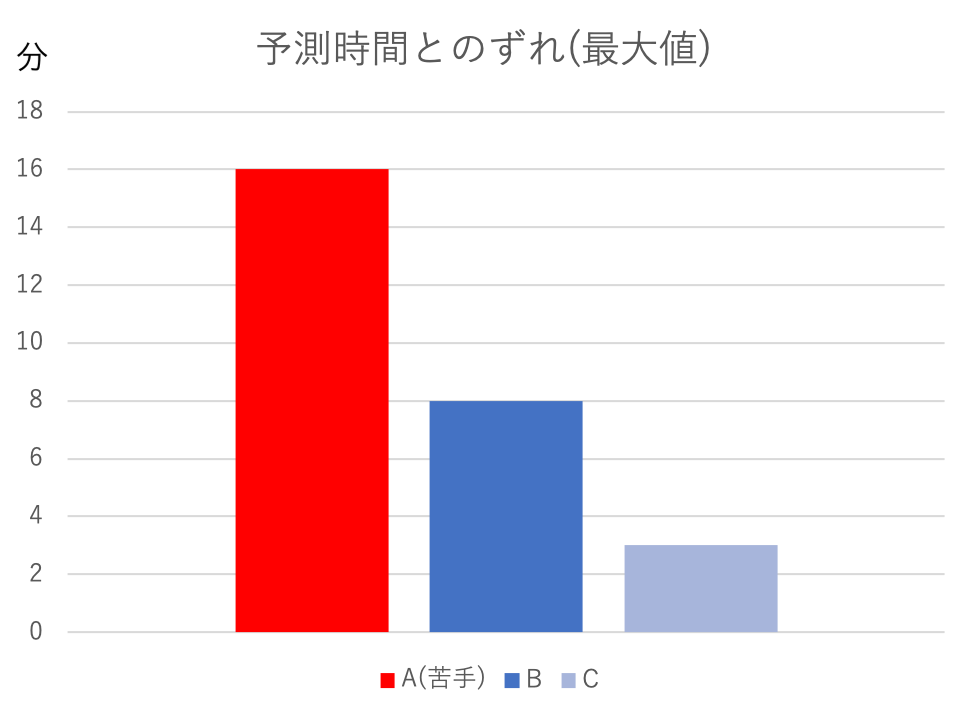
\includegraphics[width=5cm]{images/3/1.png}}
		\caption{被験者結果(最大値)}
		\label{fig:re1}
	\end{center}
  	\end{minipage}
	\\
		\begin{minipage}[b]{0.5\linewidth}
	\begin{center}
		\fbox{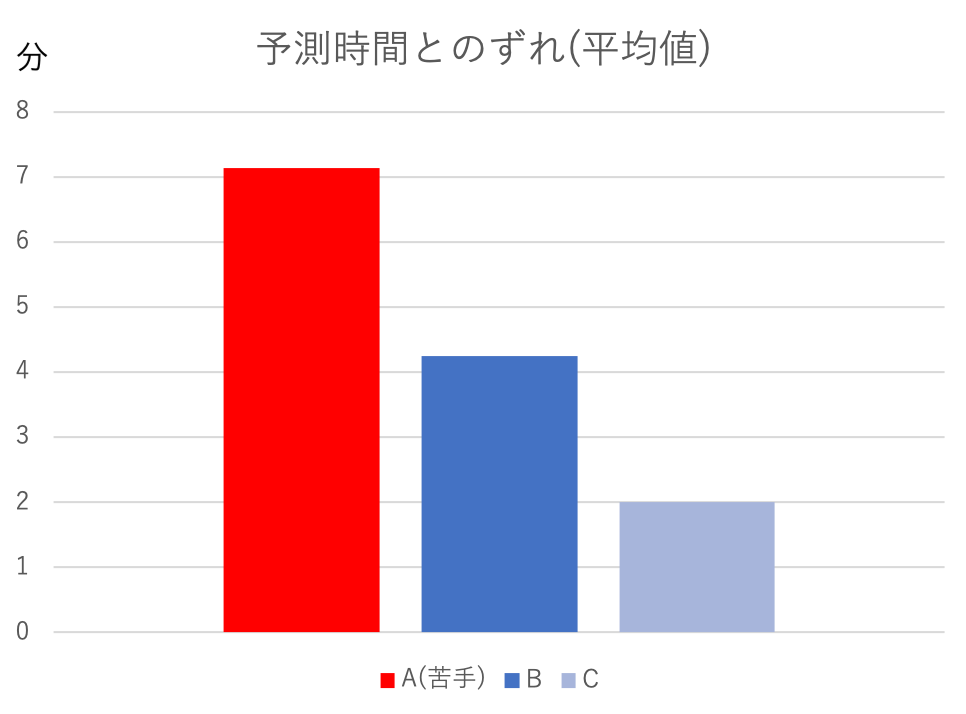
\includegraphics[width=5cm]{images/3/2.png}}
		\caption{被験者結果2}
		\label{fig:re2}
	\end{center}
  	\end{minipage}

\end{tabular}
\end{center}
\end{figure}

また,被験者によっては時間の計画の時点から不備が発生している日もあった.Bにおいては日常生活動作毎の予測時間の合計が予想準備時間(支度開始見込み時刻 - 第一理想時刻)を超えており,計画面から間に合わない計画を立てていた.(事実その日は第一理想時刻には間に合わず,第一理想時刻と第二理想時刻の間に外出していた.)

\subsection{狙い}
実験結果から,「逆算が苦手」の定義は複数人規模のプロジェクト管理でも言及されていた事と同様に,各タスク見込み時間を実態より短く認識している「見積もり時間の誤差の大きさ」場合とタスク見込み時間の総時間と総準備時間の認識が合致していない上に不十分な予備時間の確保である「バッファの不備」が原因である場合が考えられる.更に破綻したデータは苦手意識のないグループで発見された為,本人の苦手意識にか関わらず被験者の時間管理能力を把握していく必要があると考えられる.
一方で,本予備実験においては被験者数・有効データ数共に少なく,更なる実験が必要であると考えられる.

本研究では,「逆算が苦手」の定義をデータを用いて更なる分析を進めると共に,主要な原因であると考えられる時間管理の見積もり精度に起因された逆算の甘さをiOSアプリケーションを用いて補正する事で時間管理に関する心理的負荷及び逆算精度の改善を図る.


\section{タスク別時間記録システムADLogger}
ADLoggerはユーザの行動名別に経過時間を記録するiOSアプリケーションである.
ユーザは行動名毎に行動時間をストップウォッチで記録できる.
予測算出画面では,行動別の平均時間がリスト形式でカラム毎に出力される.
カラムを複数選択する事で複数行動を行う際の必要時間を計算・可視化する事が可能である.
ADLoggerが特徴とする機能には以下のものが挙げられる.

\subsection{タスク別ストップウォッチ記録}
内蔵されているストップウォッチで行動名毎に行動時間を実測で記録される.
実測値を記録する為,個人の見積もり精度に依らない数値を取得することが可能である.

\subsection{各時間予測}
各行動を下記の計算方法を用いてユーザの行動別記録時間の標準的な時間を算出し,リスト形式で行動別に表示する.
リストのカラムをタップすると,選択された行動の合計の必要時間を下記の計算手法を元に算出する.
これにより簡単に複数タスクに対する必要時間見込みを簡単に把握する事が可能となる.
算出された合計時間はAppleのカレンダーに登録が可能であり,Appleカレンダーに登録された既存の予定と同時に閲覧することが可能である.

\subsection{各時間予測の算出}
タスク完了に要する時間の期待時間を$\bar{T}$,記録時間を$T$とすると,数式(\ref{T})の様に平均時間を用いて各タスクの見積もりを行う.
また標準偏差の信頼範囲に則り,各タスクの標準偏差$s(T)$に$N$を掛けたものを変動バッファ$Tv$と定義した(数式(\ref{Tv})).
\begin{equation}
\label{T}
\bar{T}=\frac{1}{n}\displaystyle\sum_{i=1}^{n}T_{i}
\end{equation}

\begin{eqnarray}
\label{Tv}
Tv=s(T)*N \\
(N= 0, 1,2, 3 )\nonumber
\end{eqnarray}

\subsection{合計時間の算出}

合計時間の予測を出すにはまず先ほど算出したタスク毎の$\bar{T}$と$Tv$し,更にユーザが自分で決定し数値として入力ができる固定バッファ$Tf$を足す事で算出する(数式(\ref{Ts})).
\begin{equation}
\label{Ts}
T_{sum}= \displaystyle\sum_{i=1}^{n} (\bar{T}_{i} + Tv_{i})+Tf
\end{equation}


\begin{figure}[ht]
\begin{center}
\begin{tabular}{c}

	\begin{minipage}[b]{0.5\linewidth}
	\begin{center}
		\fbox{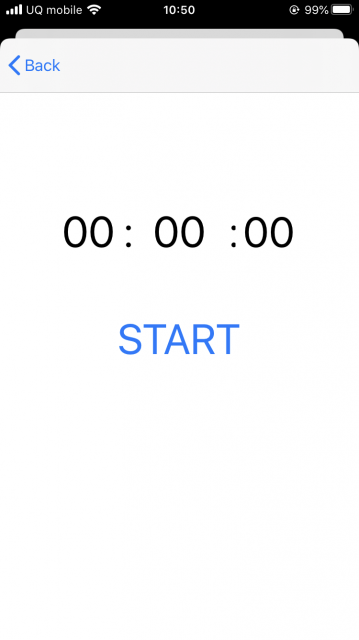
\includegraphics[width=5cm]{images/4/stopwatch.png}}
		\caption{ストップウォッチ画面}
		\label{fig:stopwatch}
	\end{center}
  	\end{minipage}
	\\	
	\begin{minipage}[b]{0.5\linewidth}
	\begin{center}
		\fbox{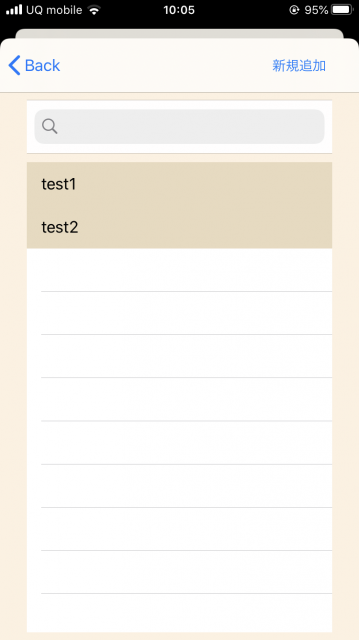
\includegraphics[width=5cm]{images/4/list.png}}
		\caption{タスク選択画面}
		\label{fig:list}
	\end{center}
  	\end{minipage}
	
  	\end{tabular}
  \end{center}
\end{figure}

\begin{figure}[ht]
\begin{center}
\begin{tabular}{c}

	\begin{minipage}[b]{0.5\linewidth}
	\begin{center}
		\fbox{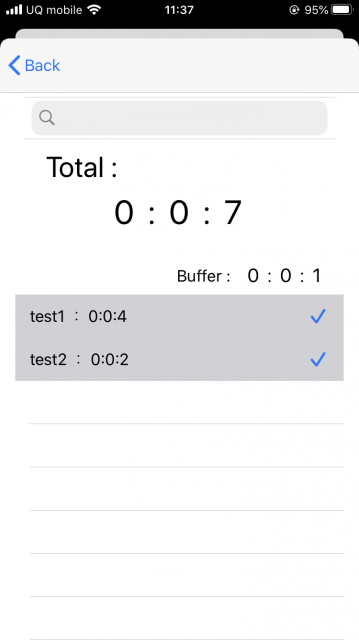
\includegraphics[width=5cm]{images/4/log.png}}
		\caption{ADLog計算出力画面例}
		\label{fig:log}
	\end{center}
  	\end{minipage}
\\
	\begin{minipage}[b]{0.5\linewidth}
	\begin{center}
		\fbox{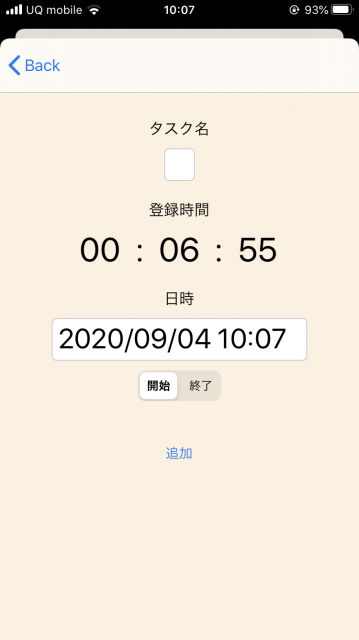
\includegraphics[width=5cm]{images/4/calendar.png}}
		\caption{カレンダー登録画面}
		\label{fig:calendar}
	\end{center}
  	\end{minipage}
	
  	\end{tabular}
  \end{center}
\end{figure}


\section{評価実験}
複数タスクにかかる所要時間に対し被験者の予測とADLoggerの予測の差異を比較した上で,
ADLogger導入によって,行動・意識の変容が生じるかどうか検証を実施した.
本章ではまず実験の目的と手法を説明し,得られた実験結果のデータの概要を示す.

\subsection{実験目的}
本研究では,複数タスクにかかる所要時間の予測に関して被験者の予測とADLoggerの予測の差異を比較し,
ADLogger導入における時間管理に対する行動の変化を目的としている.

\subsection{実験手法}
今回の評価実験では,被験者に時間の長さを教示し,その長さを産生させる時間産生法\cite{Oguro1961}を慶應義塾大学の学生男女20名に対し平日と休日(またはそれに準ずる日)にそれぞれ3回(合計6回)に渡って実施した.
始めに,被験者は事前に各自保持しているiPhoneにADLoggerをインストールして貰う.

実験は平日と休日(またはそれに準ずる日)は異なる動き・見積もりを行う可能性を鑑み,3回分の平日と休日をそれぞれ1回ずつ以上(計6回以上)実施した.
被験日はまず行動前に朝実施する日常生活動に関して行動名,行動毎の必要時間予測,タスクを連続で行った時の総合必要時間予測を申告してもらう.
尚,6回の計測を通じて予測を適宜修正できるものとする.
その後,web会議ツールであるzoomおよびADLoggerを用いながら実際に行動して貰い実測値を計測する.
zoomにおいては全ての行動の開始時/終了時に連絡を行い,実験者が総合時間を計測する.
更に被験者はADLoggerを用いて行動毎の時間を計測する.
一定期間後(原則4回目)以降の計測はADLoggerのADLogおよびタイマーのカウントアップ表示を閲覧できる状態にしながら計測して貰う.

\subsection{評価手法}
本研究はTableauを用いて下記の通り評価を行う.
アプリケーションの介入によって見積もりと実測の差がどれだけ変化したか分布の俯瞰及び平均・標準偏差を用いて全体の比較を行う.

\subsection{結果}
被験者20名中,被験に協力頂いたのは19名だった.
内,被験期間内に実験を終わらせられた(被験回数6回以上,ADLogの効果比較済)のは16名だった.

また,被験者が行う行動・行動時間は被験者に合わせている為,行動時間には個人差がある.
図~\ref{fig:day}上部はタスク別,下部は合計時間の分布を箱髭図で描いたものであり,被験者の行動時間は個人差が大きいことが分かる.

さらに,ADLog 導入前の予測と実測の平均時間の比較を 切片が 0 の一次関数で表すと,タスク別予測と実測の平均 時間の比較は y=0.96x,総合時間は y=0.99x になった.この 事から被験者 を全体で見ると予定の予測をぴったりかや や実測より短めに見積もる傾向がある事が分かる.係数は タスク別で 1.93 から 0.69 の間で,総合時間は係数 1.55 か ら 0.73 の間で見積もっていた.

箱髭図の分布を図~\ref{fig:10}にて表した.
図~\ref{fig:10}はタスク時間の秒数での分布,\%での分布,総合時間の秒数での分布,\%での分布を表しており,それぞれADLog導入前後の分布である.
また図~\ref{fig:10}の平均値・標準偏差を表~5で表した.表~5で分かる通り全ての分布はADLog導入後の方が分布が狭まった事で標準偏差が小さくなっている.
尚,ADLog導入後に見積もりの時間を変更したのは3人である.

\begin{table*}[tb]
\setbox0\vbox{\large

\begin{center}
\caption{導入前後比較}
\ecaption{Comparison before and after}
\begin{tabular}{|c|c|c|c|c|} \hline
 & タスク時間(秒) & タスク時間(\%) & 総合時間(秒) & 総合時間(\%) \\ \hline 
平均(導入前)& 28.12& 136.59 & -21.37& 105.89 \\ \hline
平均(導入後)& 20.46& 121.24 & -49.89& 100.98 \\ \hline
標準偏差(導入前)& 193.02& 102.47 & 460.50& 29.10 \\ \hline
標準偏差(導入後)& 169.93& 62.55 & 356.20& 25.37 \\ \hline
\end{tabular}
\label{tb:9}
\end{center}
}

\centerline{{\hbox to.9\textwidth{\hss\box0\hss}}}
\label{tb:dif}
\end{table*}



\begin{figure*}[tb]
\setbox0\vbox{\large
\hbox{\
	\fbox{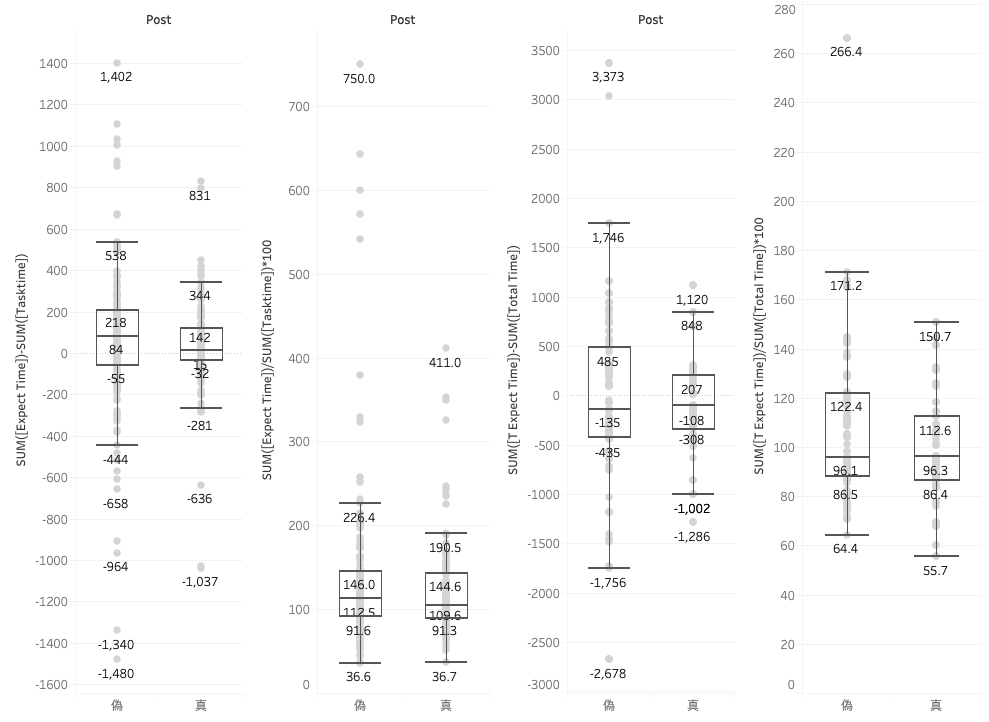
\includegraphics[width=15cm]{images/7/10.png}}
}}
\centerline{{\hbox to.9\textwidth{\hss\box0\hss}}}
\caption{ADLog導入前後の比較(箱髭図)}
\ecaption{Comparison before and after system introduction.}
\label{fig:10}
\end{figure*}

\section{考察}
実験結果から,ADLog機能導入によって見積もりの予測時間と実測時間の差が縮まる効果が得られた.特に時間管理に対し苦手意識のある被験者や見積もりの係数が1に近い被験者程効果が大きかった.
一方,ADLog導入後に見積もりの時間を変更した人はわずか3人である点から本アプリケーションは
「見積もり傾向から自分の精度の悪い見積もりを修正する事によってズレが少なくなる」のではなく,「時間傾向の可視化に対しタイマーのカウントアップによって時間をより合わせる」効果をより発揮していると考えられる.

また,傾向線で見ると下振れしている被験者が多い事から,本機能の用いたバッファの取り方では見積もりを少なく見積もる様になってしまう可能性があり,バッファや目標時間は本機能の提示では正しく導けない事が分かる.
これは被験者別に傾向のタイプ分けをせず,かつまだ前例の無い中での暫定的な見積もりの提示をしており,より最適化が求められると考えられる.

\section{今後の展望}
\subsection{ADLogger}
ADLoggerの導入前後で予測時間とのズレが少なくなったと述べたが,これは実態時間が予測時間より長い時だけでなく短い時も同様に発生する.
つまり被験者によっては無意識に時間にゆとりを持っていたにも関わらずADLogger導入によってバッファが短くなってしまう可能性が発生する.
バッファの短縮を阻止し,最適な時間を提案する為には本実験で用いた計算手法の改善やユーザ別もしくはユーザのタイプ別に計算手法を変えていく機能が必要であると考えられる.

また,改善すべき点を被験者に伺ったところ,多くの改善案が提案された為,少しずつ改善していく必要がある.
まず短期的なUI改善においては検索機能の搭載やタスク登録後自動的にタイマーが面に戻る機能,ルーティンのオンオフの切り替えの簡易化などが挙げられた.
またタスク登録にて提示される登録タスク候補はサーバに保管されたタスクと同期していない点や自分の設定がADLog画面でしか確認が難しい点が問題点に上がった.
長期的なUI改善としては音声の指示,トラッキングと言った計測の負担を減らす手法が提案された.

\subsection{実験環境}
本実験では被験日には実験者とzoomで話すというプロセスが組み込まれている.
カメラオフ・実験中はマイクオフで参加可能であるとしたものの,実験の度に実験者と会い,
実験終了まで実験者が待っているという環境はそれだけでも必要以上に実験の存在を意識する可能性がある.

また,実験は実際に普段行っている朝の支度を再現してもらった為,一人一人行った作業は異なる.
加えて実験した場所はそれぞれの自宅なので環境が異なる場合がある.
例えば実家暮らしだと一人暮らしの被験者とは違い他の家族の行動によって時間をずらす必要が生じる.
特に実験中に引越しした被験者がおり,一部の被験者はルーティンの変化などに影響がある可能性がある.
この事から行うタスクを均質にして同環境下で実験する必要性が考えられる.

\subsection{評価手法}
今回の実験は短期間かつ少人数で実施した為,アプリケーションの普遍的な効果を本実験・データ数のみで評価することは厳しいと考えられる.
この為被験者人数と日数はより増やした検証を行う必要がある.
特に「逆算が苦手である為時間管理が難しい」人を絞り込み,効果検証を行えばもっと精度の高い評価が得られる可能性がある.

また評価に関して今回の実験はy=axの傾向線を用いて行ったが,そもそも見積もりの予測傾向に関する理想のモデルは線形とは限らない.
予測傾向に関するモデルの先行研究が存在しない為,今後実験を通して最適な傾向モデルを模索していく必要がある.

最後に今回はルーティンに対する慣れの因子がより強く出ていたが,本来は情報処理能力と多次元処理能力と言った「マルチタスク」に関する能力\cite{multitask}や時間感覚\cite{Tayama2018}の個人差による違いも出る可能性がある.
先ほどあげた因子の他にも時間の見積もり自体は個人間でも均一になりにくい事など偏り及び多くの交絡因子が考えられ,時間把握の能力策定には更なる収集が必要である.

\section{本論文のまとめ}
本論文では,タスク毎の時間及び合計時間の見積もり精度を向上させるためにADLoggerを提案・実装した.
ADLoggerはストップウォッチで記録されたでタスク毎の時間を基にユーザの行動時間傾向を予測し必要時間見積もりを簡単に導き出せるアプリケーションである.
評価実験は総勢19名の被験者に協力頂き朝の準備支度を想定した環境でADLoggerを使ってもらい評価実験を行った.
結果見積もりの時間と実態の時間のばらつきを縮小させた事が示唆された.
一方で被験者によっては余裕がある予測時間を削る方向で縮小させてしまったり,個人差の大きさなどが問題点として残った.
今後はユーザのタイプに合わせた機能の変化や見積もりの時間の最適化が求められる.
\bibliographystyle{unsrt}
\bibliography{bibsample}
\end{thebibliography}

%4.6
\acknowledgment
本研究はJSPS科研費JP19K20260の助成を受けたものである.本研究はJST,CREST,JPMJCR19A4の支援を受けたものである.

\end{document}
